\documentclass[a4paper,openright,12pt]{article}
\usepackage[utf8]{inputenc}
\usepackage{graphicx} 
\usepackage{subfigure}
\usepackage[mathscr]{eucal}
\usepackage{titling}
\usepackage{float}
\usepackage{amsmath}
\usepackage{afterpage}
\usepackage{vmargin}
\usepackage[spanish]{babel}
\usepackage{eurosym} 
\usepackage{multirow} 
\usepackage{cite}
\usepackage{url}

\setpapersize{A4}	   %  DIN A4
\setmargins{3cm}    % margen izquierdo
{3.5cm}                     % margen superior
{15cm}                       % anchura del texto
{22.5cm}                   % altura del texto
{10pt}                         % altura de los encabezados
{1cm}                         % espacio entre el texto y los encabezados
{0pt}                           % altura del pie de página
{2cm}                         % espacio entre el texto y el pie de página

\begin{document}

\begin{titlepage}

\begin{center}
\vspace*{-1in}
\begin{figure}[htb]
\begin{center}

\includegraphics[width=8cm]{udc.eps}
\end{center}
\end{figure}

\vspace*{1in}
PROGRAMACIÓN DE SISTEMA 21/22 Q1\\
\begin{center}
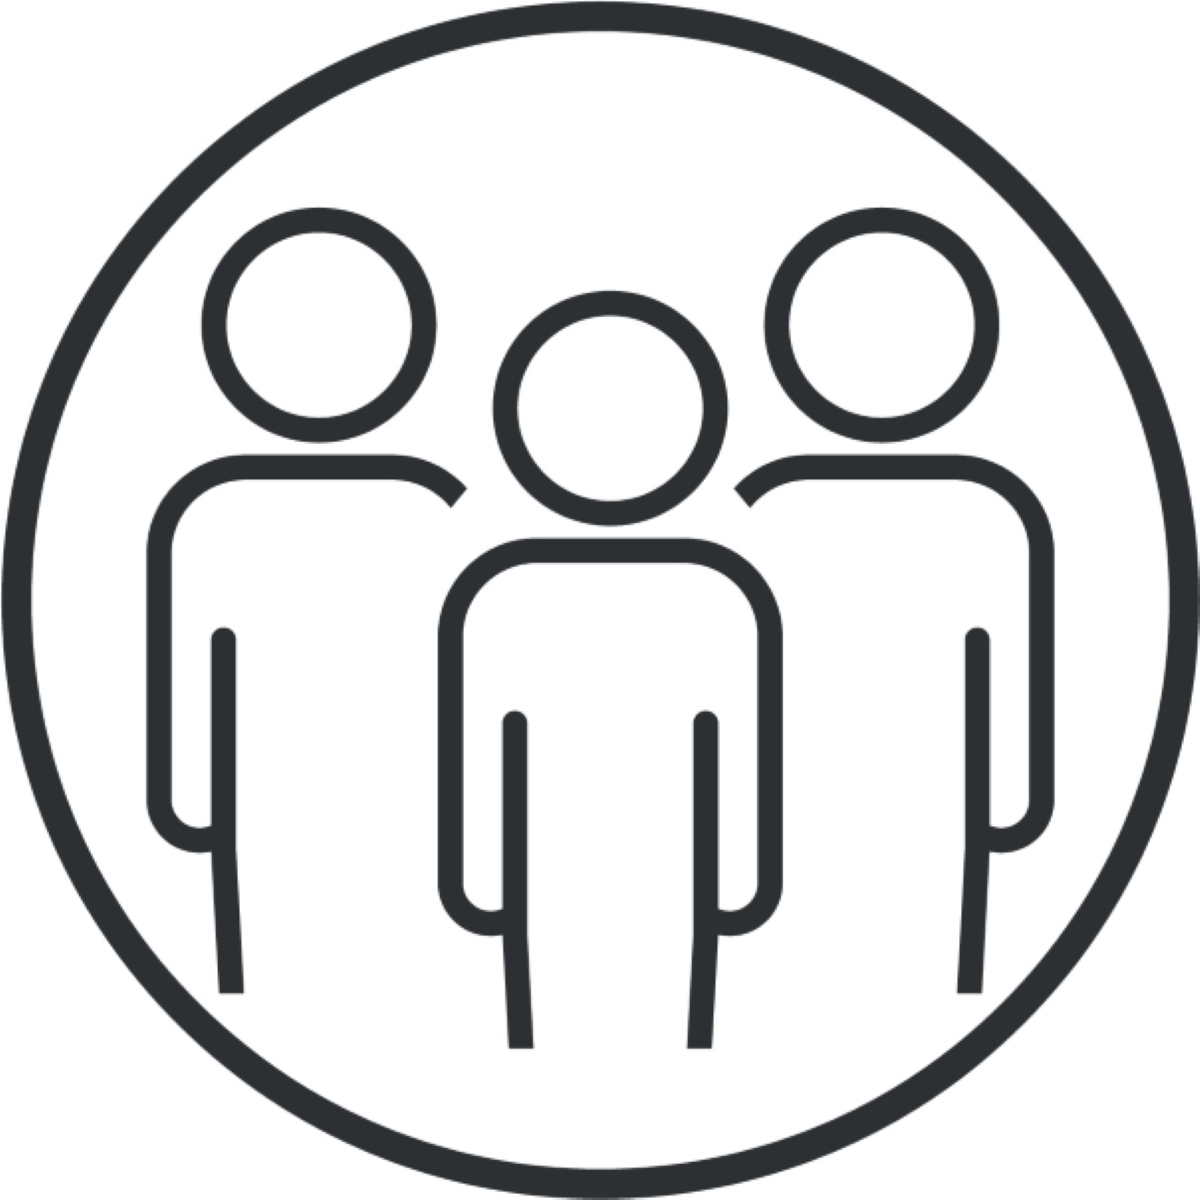
\includegraphics[width=3cm,height=3cm]{ejemplo.jpg}
\end{center}
\vspace*{10mm}
\begin{Large}
\textbf{Desarrollo de una aplicación de control de aforo en Android} \\
\end{Large}
\vspace*{10mm}
\begin{Large}
\textbf{Portiñas} \\
\end{Large}

\vspace*{3in}
\begin{large}
\raggedleft
\textbf{Autores:} Brais Barboza Ordoñez\\
Julián Barcia Facal (julian.bfacal@udc.es) \\
\textbf{Fecha:}\textit{A Coruña, 13 de enero 2022}\\
\textbf{Versión:}\textit{3.0}\\

\end{large}

\end{center}
\end{titlepage} 

\newpage

\addtocontents{toc}{\hspace{-7.5mm} \textbf{Capítulos}}
\addtocontents{toc}{\hfill \textbf{Página} \par}
\addtocontents{toc}{\vspace{-2mm} \hspace{-7.5mm} \hrule \par}

\pagenumbering{empty}

\tableofcontents

\vspace{3cm}

\begin{flushright}
\begin{table}[hbtp]
\begin{center}

\caption{Tabla de versiones.}
\label{tabla:versiones}
\small
\vspace{1ex}

\begin{tabular}{|c|c|l|}
    \hline
    Versión & Fecha & Autor \\
    \hline \hline
    1.0 & 06/10/2021 & Julián y Brais\\ \hline
    2.0 & 09/11/2021 & Julián y Brais\\ \hline
    3.0 & 13/01/2022 & Julián y Brais\\ \hline
\end{tabular}

\end{center}
\end{table}
\end{flushright}
\newpage
\pagenumbering{arabic}

\section{Introducción}\label{cap.introduccion}
Esencialmente la aplicación controlará el acceso del personal de un edificio. Con una estación de control en cada acceso, el personal de forma casi transparente podrá acceder al edificio o marcharse del mismo.
El personal contara con un dispositivo con la tecnología NFC (mismamente su teléfono) el cual a la hora de entrar al edificio escanearan contra la aplicación de la puerta, que les garantizara el acceso en caso de cumplir los requisitos necesarios.

%%
\subsection{Objetivos}
El objetivo principal de este trabajo es gestionar el control de acceso de un edificio o recinto genérico, de tal modo que se tenga un control del número de personas que entran y salen de dicho recinto. Además, buscaremos también crear un lector de identificación, de tal modo que cada usuario pueda ser reconocido de manera individual e inequívoca. De esta manera mediante un teléfono, a través de la app, podremos agilizar los trámites de aforo y acreditación.
%%
\subsection{Motivación}
Debido a la situación de pandemia en la que nos encontramos el control de aforo se ha vuelto un requisito indispensable en muchas ocasiones para poder cumplir las legislaciones continuamente cambiantes. Esta aplicación busca servir, de una manera simplificada, como ayuda para cubrir estas nuevas necesidades que la pandemia ha generado consigo.

%%
\subsection{Trabajo relacionado}
Antes de realizar este trabajo se ha buscado información sobre otros proyectos similares, con objetivos y motivaciones similares a las nuestras o que simplemente nos sirvan como un punto de referencia para nuestro diseño.
En un primer lugar nos centramos en tener una idea general de lo que podría abarcar este tipo de proyecto. Tomando como referencia otros trabajos \cite{TFG_bares}, se ha conseguido clarificar cuáles pueden ser los requisitos e incidencias, a pesar de que el producto final no sea exactamente como el nuestro. \par
Una vez sentadas las bases, se ha hecho uso de proyectos que nos sirvieran como clara referencia para nuestra implementación. Ideas para una interfaz de mayor sencillez y accesibilidad o como hacer un almacenamiento de los datos de forma más eficiente han sido ideas que se han consultado en \cite{TFG_complu}. \par
Dado que se va a hacer uso de una base de datos en tiempo real, en concreto la que nos proporciona \textit{Firebase}, se han indagado sobre posibles trabajos que tuvieran el uso del servicio de \textit{Firebase} y su base de datos como objetivos principales. De este modo el trabajo de Marina Castellote García \cite{TFG_apuestas}, ha servido como buena referencia para estas labores. \par
Por último, como buscamos que nuestro sistema sea capaz de utilizar el sistema de RFID para la identificación de usuarios a su entrada y salida del aforo, el trabajo de Marcos Manuel Gallego Ferrer \cite{Safe-Events}, es una gran referencia no tan solo por su descripción e implementación de los sistemas de RFID ya mencionados sino también por las grandes similitudes en el producto final y objetivos que se pretenden obedecer.


%%%%%%%
%%%%%%%
\section{Análisis de requisitos}
%%
\subsection{Funcionalidades}
La aplicación como funcionalidad central tiene el control de aforo de un recinto. Si bien esta idea es bastante simple en un primer momento, la esencia del proyecto reside en su implementación. Sobre un método clásico, como un usuario controlando manualmente el aforo con la ayuda de la app, se proponen una serie de funcionalidades que se implementarán de forma progresiva:
\begin{itemize}
    \item Posibilidad de configurar el edificio, controlando las entradas y las salidas además del aforo
    \item Actualizar el estado (entrada o salida) del sistema mediante dispositivos móviles con tecnología NFC.
    \item Mantener un histórico a disposición de la administración de los accesos y salidas del recinto.
    \item Identificar cada histórico con un valor único, pudiéndose acceder a ellos mediante el uso de este.
    \item Posibilidad de borrar y cambiar de base de datos y su identificador, teniendo otra automáticamente, completamente nueva y con otro identificador.
    \item Informar al usuario en su dispositivo en caso de que un intento de acceso haya sido denegado.
\end{itemize}

%%
\subsection{Prioridades}
El proyecto tiene como idea central la escalabilidad del mismo. Siendo una idea sencilla permite una alta cantidad de incrementos en función de los requisitos de una organización. Por ello las prioridades serán:
\begin{enumerate}
  \item Crear un histórico local en un único acceso mediante un único terminal de forma manual.
  \item Implementación de un sistema de sincronización entre varios terminales para pasar a tener un histórico combinado, ampliando así el posible número de entradas y salidas, además de que el histórico está almacenado en \textit{cloud}.
  \item Identificación de cada sistema de manera única de tal modo, que se pueda conectar a su base de datos en cualquier momento con el uso de su identificador.
  \item Implementación de una aplicación para el acceso mediante dispositivos individuales, permitiendo el control en varios accesos de modo automático.
  \item Registro de intentos de acceso y salida.
\end{enumerate}

Cabe destacar que independientemente de las prioridades previamente descritas, el proyecto pretende aumentar de tamaño capa a capa, de forma que cada nivel individual sea plenamente funcional por sí mismo.
%%%%%%%
%%%%%%%
\section{Planificación inicial}

%%
\subsection{Iteraciones}
\begin{enumerate}
    \item Implementar una aplicación que muestre el aforo en el momento actual e incremente o decremente de manera manual, según las personas salgan o entren.
    \item Utilizar NFC \cite{NFC} para ser capaces de identificar a cada persona que entre de manera individual.
    \item Conseguir que este recuento se haga de manera automática al detectar la entrada y salida de usuarios.
    \item Hacer uso de una base de datos en tiempo real, de tal modo que los accesos y salidas se contabilicen en linea, de forma que el aforo esté actualizado y sincronizado de forma simultánea en varios puntos de acceso y salida. 
    \item Mantener un registro de accesos al registro a nivel individual.
    \item Posibilidad de creación de grupos con franjas horarias de accesos.
\end{enumerate}

%%
\subsection{Responsabilidades}
La estructura del proyecto y la repartición de tareas se han hecho de la siguiente manera:

\begin{enumerate}
    \item La creación del modelo inicial, compuesto por un contador que guardaba sus datos en modo local, y con un funcionamiento plenamente \textit{offline} a quedado a cargo de Julián.
    \item La extrapolación de este modelo a un contexto en línea, mediante el uso de una base de datos en tiempo real \textit{(Firebase)} ha quedado a cargo de Julián.
    \item La identificación de cada empleo de la aplicación, con un código único y el cual se vincula con una base de datos propia en \textit{cloud} ha sido implementada por Julián.
    \item La identificación de cada dispositivo, mediante el uso de NFC ha quedado a cargo de Brais. 
    \item La adaptación de la aplicación a un esquema como el
    \textit{Model View Controller} ha quedado a manos de Brais.
    \item El desarrollo de una capa \textit{front-end}, sencilla y entendible para un nuevo usuario se ha hecho de forma conjunta, ayudándose de \textit{testers} o terceros, teniendo su interacción con la aplicación como referencia para cambios significativos.
    \item La actualización de este documento se ha hecho de manera mutua, añadiendo cada uno de los integrantes aspectos y matices reseñables, a medida que se avanzaba en el desarrollo del proyecto.
\end{enumerate}

%%
\subsection{Hitos}
El desarrollo del proyecto se va a organizar en \textit{sprints}. Este modelo es el que más se adapta a la idea inicial de nuestro proyecto. Además, su uso compagina en gran medida con el uso de \textit{git-flow} y su modelo de control de versiones. Cada Sprint en nuestro caso se corresponderá con secciones de desarrollo importantes junto con diversos \textit{features}.

\begin{itemize}
\item{\textit{Fase de planificación:} Esta fase se centrará en crear una primera versión del proyecto, diseñando de manera esquemática funcionalidades e interfaz que serán utilizadas próximamente. En esta sección se incluye también la creación de este documento, que será actualizado a lo largo del proyecto}
\item{\textit{Fase de desarrollo de la aplicación \textit{offline}:} Esta fase centra el foco en integrar las funcionalidades y el diseño de la anterior iteración. Al final de esta etapa, se podría un realizar un test para comprobar el correcto funcionamiento de las funciones principales de la aplicación. El test se hará de manera manual, sobre un dispositivo físico, para evitar errores que puede ocultar el emulador.}
\item{\textit{Integración de base de datos en tiempo real:} En este apartado se busca que una vez construida la base sobre un modelo
local, consigamos transmitir los datos a una base de datos en \textit{cloud}. El correcto funcionamiento de este se hará tanto en el dispositivo como a nivel \textit{online}. A nivel local los cambios efectuados deben de seguir siendo visibles. A su vez, los datos deben sufrir los mismos cambios en la base de datos en tiempo real y estos se deben poder consultar con el simple uso de un navegador web.}
\item{\textit{Identificación y conexión de dispositivos:} Buscaremos en este apartado que cada ejecución de la aplicación cuente con un código único vinculado también a su propia base de datos en tiempo real. Con el conocimiento de este código, se debe permitir también la conexión entre dispositivos de tal modo que sincronicen sus datos en una única base de datos.}
\item{\textit{Integración del sistema de lectura:} Esta sección se focalizará en integrar el método de NFC en las funcionalidades de la aplicación. Al finalizar esta tarea se podría realizar un test para comprobar la correcta lectura y reconocimiento de los dispositivos.}
\item{\textit{Información de la petición en el dispositivo individual:} Informar al usuario de si su intento de acceso ha sido aprobado, o de la denegación del mismo con una explicación breve.}
\item{\textit{Pruebas:} A medida que se avanzaba en la parte de desarrollo, se realizarán pruebas para verificar el funcionamiento del modelo planteado y comprobar con qué ajustes sería más óptimo. Paulatinamente se intensificarán las pruebas para poder obtener una mayor cantidad de datos y así poder decidir que avances priorizar. Al finalizar el desarrollo total, se realizarán pruebas de resistencia para comprobar la estabilidad del sistema}
\item{\textit{Posibles nuevas funcionalidades y cierre del proyecto:} Esta última sección se centrará en añadir nuevas tareas, pero de pequeño tamaño que no pueden comprometer el cierre final del proyecto. Esta última tarea viene acompañada de pruebas sobre el funcionamiento completo de la aplicación.}
\end{itemize}

%%
\subsection{Incidencias}
Si bien la naturaleza del proyecto es simple en planificación, el desarrollo de un sistema completo puede resultar de mayor dificultad de la prevista. Estos problemas se traducen en unos retrasos en las planificaciones debido al aumento de los tiempos dedicados a cada tarea. 
De este modo, durante el desarrollo de este proyecto se han producido una serie de incidencias:
\begin{itemize}
    \item \textit{Uso de ProgressBar:} Durante la realización de este proyecto, para crear una interfaz más visual como se ha dicho la cuenta del aforo se acompaña de un círculo dinámico. El problema encontrado con este elemento es su implementación debido al desconocimiento previo de su funcionamiento para el equipo de desarrollo. Variantes fuentes \cite{ProgressBar_developer}, \cite{ProgressBar_develou} serán empleadas para solventar este cometido.
 \item \textit{Uso de Real Time Database:} Para la implementación síncrona del programa, se necesita hacer uso de una base de datos en tiempo real \cite{Firebase_DOC}, al igual que el caso anterior, el equipo de desarrollo no cuenta con conocimientos previos por lo cual se debe utilizar cierto tiempo en su aprendizaje.
     \item \textit{NFC:} 
     Sumado a esto, la comunicación NFC puede traer consigo distintas problemáticas, entre ellas la más evidente: se necesitarán varios dispositivos con dicha característica para poder comprobar el funcionamiento del sistema.
      \item \textit{Ajustes:} En esta aplicación se hace uso de una sección de ajustes, implementada con una \textit{Preference Activity} y su \textit{fragment} asociado. La sincronización del campo de aforo que se muestra en dichos ajustes, con el guardado de forma inicial y con los diferentes elementos de la interfaz que deben cambiar ha resultado de mayor complicación de la prevista, produciendo retrasos en la producción.
 




%%%%%%%
%%%%%%%
\section{Diseño}
\subsection{Arquitectura}
Se diseñará el proyecto con la arquitectura CLEAN en mente.
Aprovechándonos de la orientación a eventos de Android, implementaremos un modelo vista presentador, donde un evento en el presentador, modificara la vista y llamara al modelo.
En cuanto a la sincronización entre dispositivos, se implementará mediante el uso de un servidor principal con una interfaz API REST.
%%
\subsection{Persistencia}
Como se ha comentado en un primer momento solo tenía soporte para guardar sus datos a nivel local, de tal modo que la existencia de varias entradas y salidas no se contemplaba. Con el uso de la base de datos en tiempo real, los datos de entrada, salida e identificación de dispositivo ahora se guardan en línea. Esto nos permite, por lo tanto, que varios dispositivos que se encuentran usando la aplicación tenga conexión y relación entre ellos.
\subsection{Vista}
Con respecto a la vista nuestra aplicación prioriza la simplicidad y sencillez por lo que nos centraremos en el uso de modelos presentes en multitud de otras aplicaciones, haciendo el uso de la nuestra mucho más intuitivo para el usuario:


\begin{enumerate}
\item\textbf{\textit{Splash-Screen:}} Al ejecutar la aplicación, esta muestra durante un breve periodo de tiempo un \textit{Splash-Screen} con el logo de la aplicación.
\begin{figure}[H]
     \centering
    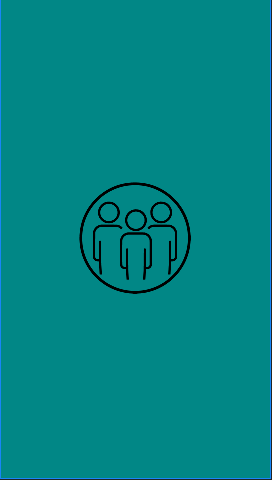
\includegraphics[scale=0.7]{splashscreen.PNG}
     \caption{Splash Screen}
    \label{fig:my_label}
\end{figure}

   
\item\textbf{\textit{Introducir aforo:}} Solo en la primera ejecución de la aplicación o si no se ha introducido un valor de aforo total todavía, la aplicación nos mostrará una pantalla correspondiente a la actividad que cubre este propósito.
\begin{figure}[H]
     \centering
    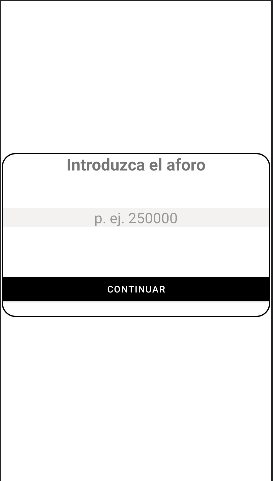
\includegraphics[scale=0.7]{Introducir.PNG}
     \caption{Introducir Aforo}
    \label{fig:my_label}
\end{figure}
\item\textbf{\textit{Fragmentos:}} Para las funcionalidades principales en esta aplicación se va a hacer uso de distintos fragmentos:
\begin{itemize}
\item\textit{Contador de aforo:} Este fragmento es el principal y es el que muestra los datos almacenados en la base de datos con respecto al aforo. Además, para mayor claridad visual se acompañan de una \textit{ProgressBar}, que nos da una idea del porcentaje de ocupación. Justo debajo se sitúan dos botones que son los que nos proporcionan las funcionalidades de registrar una salida y entrada respectivamente.
\begin{figure}[H]
     \centering
    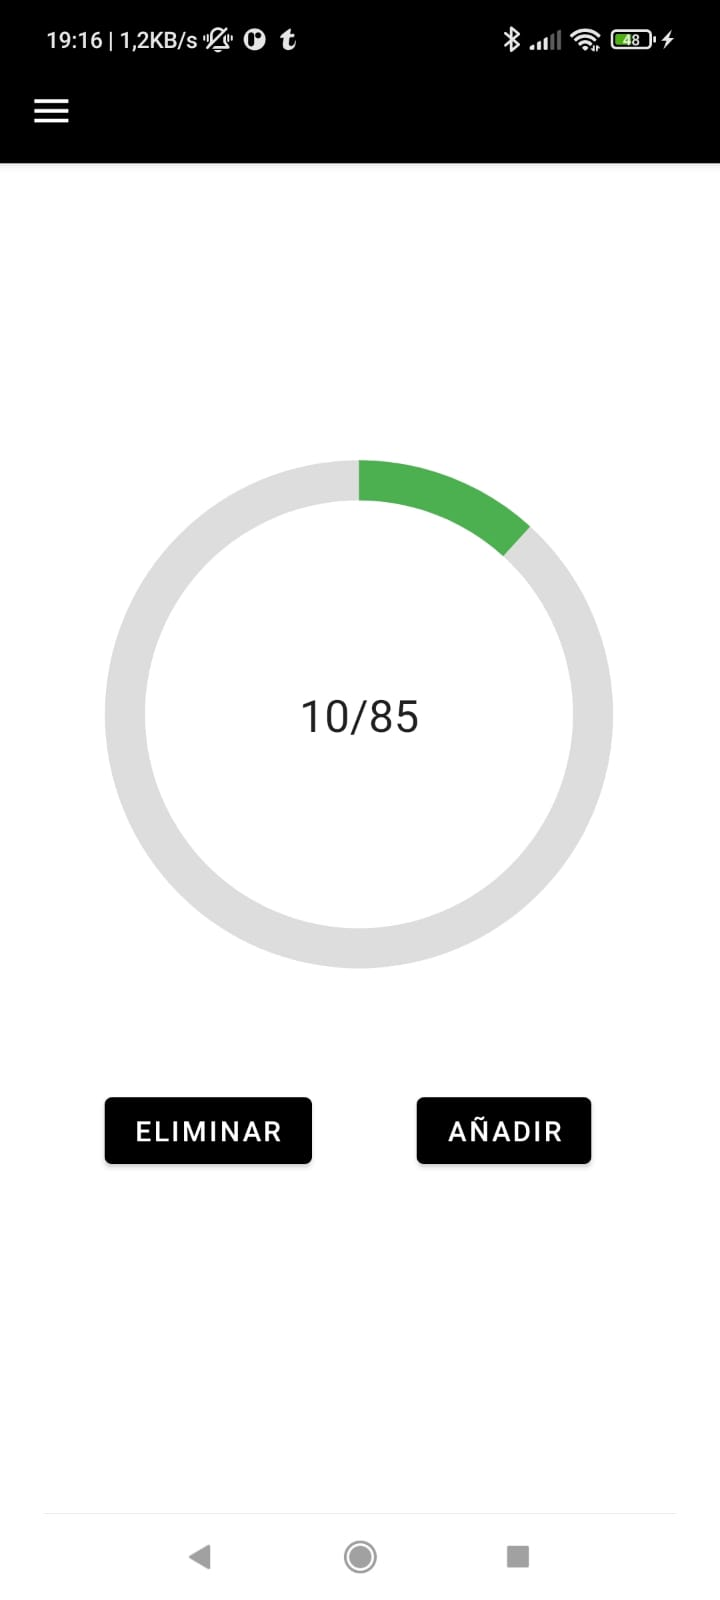
\includegraphics[scale=0.2]{aforo.jpeg}
     \caption{Fragmento con contador en tiempo real de aforo}
    \label{fig:my_label}
\end{figure}
\item\textit{Código identificador:} En este fragmento el usuario podrá ver el código que le corresponde a su dispositivo. En esta misma vista el usuario cuenta con un botón al lado de un campo rellenable. Estos permiten al usuario conectarse a otro dispositivo, a su base de datos, para sincronizar sus valores y cambios. Además, se cuenta con un botón adicional para reiniciar el identificador y su base de datos vinculada.
\begin{figure}[H]
     \centering
    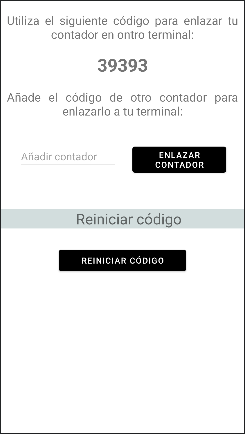
\includegraphics[scale=0.7]{CODE.PNG}
     \caption{Fragmento con código identificador}
    \label{fig:my_label}
\end{figure}
\item\textit{NFC:} En este fragmento el usuario podrá ver el código que le corresponde a su dispositivo. En esta misma vista el usuario cuenta con un botón al lado de un campo rellenable. Estos permiten al usuario conectarse a otro dispositivo, a su base de datos, para sincronizar sus valores y cambios. Además, se cuenta con un botón adicional para reiniciar el identificador y su base de datos vinculada.
\begin{figure}[H]
     \centering
    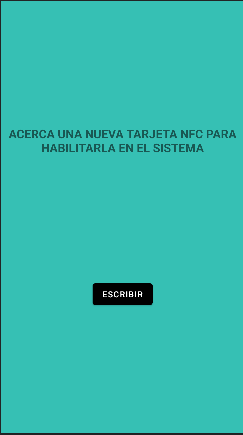
\includegraphics[scale=0.7]{NFC.PNG}
     \caption{Fragmento para conectar NFC}
    \label{fig:my_label}
\end{figure}
\end{itemize}
El botón de regreso en cualquier de estos fragmentos devuelve un Toast indicando al usuario que presionando de nuevo cerrará la aplicación.
\item\textbf{\textit{Navigation Drawer:}} Para el simplificar el acceso a los diversos fragmentos y otras funcionalidades se hace uso de un \textit{Navigation Drawer} que permite al usuario saltar entre estas distintas secciones. En él además de los fragmentos anteriormente mencionados también se encuentran:
\begin{itemize}
    \item {\textit{Ajustes}: Contamos con un fragmento adicional para ajustes. En él se puede modificar el aforo total del edificio. Al presionar el botón de regreso el usuario volverá al fragmento principal, donde podrá ver que se han realizado los cambios. En el caso de que la capacidad total que se haya introducido sea menor que el recuento del número de personas que se encuentran en el interior el sistema reinicia este recuento a 0, en el caso general simplemente modifica la capacidad manteniendo el conteo.}
     \item {\textit{Compartir}: Este elemento mediante el uso de un intent le mostrará al usuario diversas opciones para compartir el enlace del proyecto.}
     \item {\textit{Sobre Nosotros}: Este elemento derivará al usuario directamente a la dirección web de la wiki de nuestro proyecto, abriendo mediante el uso de intent en el navegador dicha página.}
         \begin{figure}[H]
     \centering
    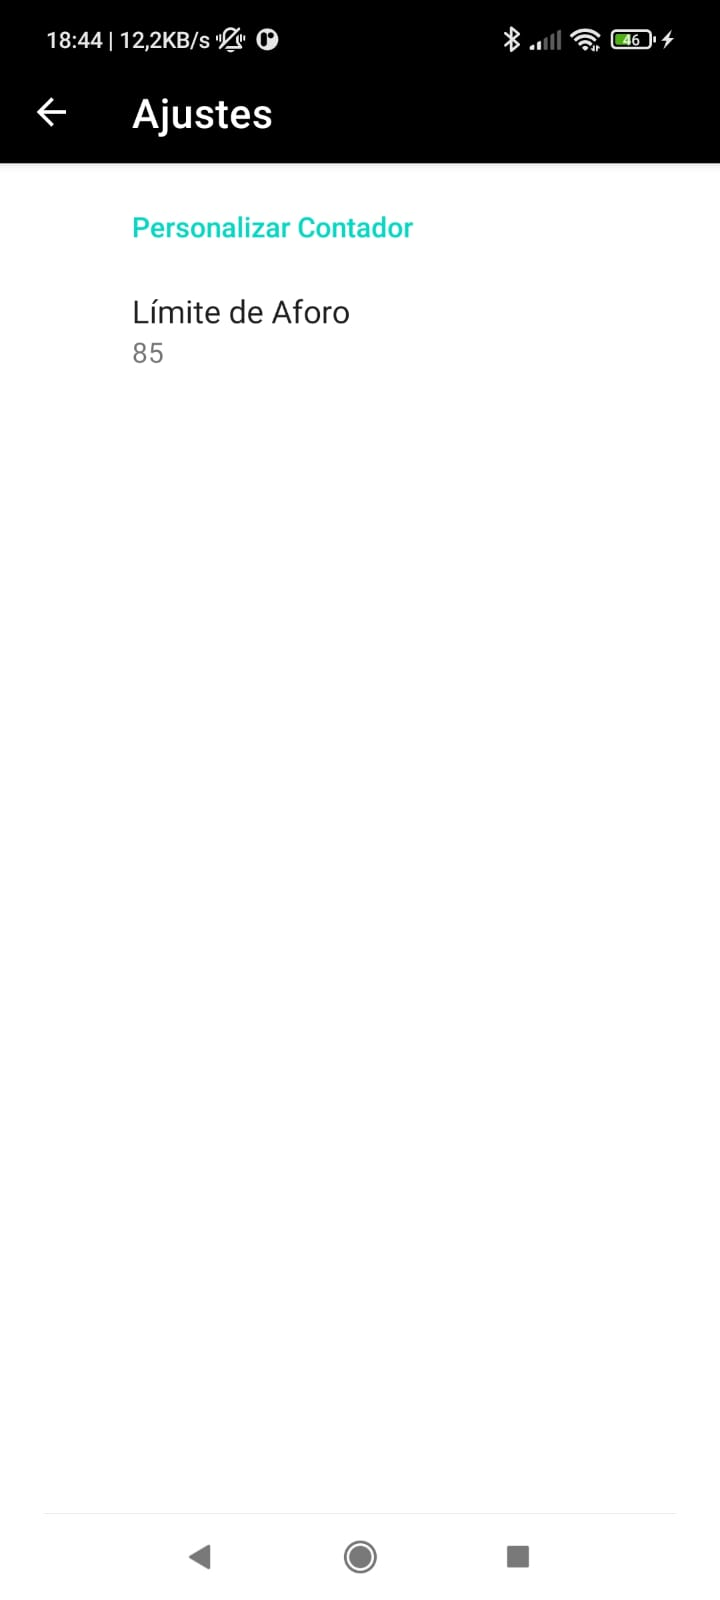
\includegraphics[width=4cm, height= 8cm]{ajustes.jpeg}
     \caption{Fragmento de ajustes para modificar aforo total}
    \label{fig:my_label}
\end{figure}
\begin{figure}[H]
\centering
\begin{minipage}{.5\textwidth}
  \centering
  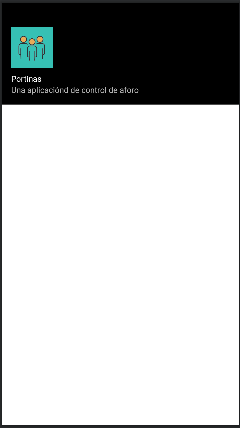
\includegraphics[scale=0.7]{header.PNG}
  \caption{Header Navigation Drawer}
  \label{fig:test1}
\end{minipage}%
\begin{minipage}{.5\textwidth}
  \centering
  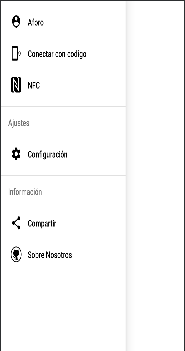
\includegraphics[width=5cm,height = 8cm]{side.PNG}
  \caption{Opciones menú}
  \label{fig:test2}
\end{minipage}
\end{figure}

\end{itemize}
\end{enumerate}

\subsection{Comunicaciones}
Para mantener una base de datos en tiempo real, en la cual podamos guardar toda la información requerida para el correcto uso de la aplicación haremos uso de {\textit{Firebase}} \cite{Firebase_Tut}, más concretamente vamos a hacer uso de su opción de {\textit{Real Time Database}} \cite{Firebase_DOC}. Como el desarrollo de esta aplicación solo tiene fines didácticos y no se pretende hacer pública, las reglas de seguridad de esta base de datos se pueden definir sencillamente como públicas, a pesar de los riegos de seguridad que esto conlleva.
\subsection{Sensores}
Para esta aplicación y más concretamente, para su funcionalidad de lectura automática, vamos a hacer uso del sensor de NFC.
Como se comenta previamente en el documento, existe la posibilidad de registrar ,los accesos y salidas al sistema mediante tarjetas NFC. La aplicación cuenta con una pantalla propia para la habilitación de las mismas que graba un identificador único en cada una, con el fin de registrar cuando esta se encuentra dentro o fuera del recinto.
En cuanto a su funcionamiento, la lectura de una tarjeta por el dispositivo, genera un Intent, que, de estar abierta la aplicación sera procesada como un ingreso.
En caso de estar en la actividad de activación, el dispositivo se pone en modo escritura, dando feedback cuando la escritura sea completada, tanto siendo correcta como fallida.
\subsection{Trabajo en background}
Ya que en Android las peticiones externas se deben ejecutar fuera del hilo principal, las interacciones con el servidor, se implementan mediante listeners.
\begin{itemize}
    \item \textit{OnComplete}: Que se ejecuta cuando se completa la petición get().
    \item \textit{OnDataChanged}: Que se llama al detectar un cambio en la base de datos actualizando los valores en pantalla de los valores asociados.

\end{itemize}
\subsection{Pruebas Realizadas}
Se ha optado por un desarrollo del testeo manual, probando las funcionalidades a medida que se implementaban, comprobando los distintos casos de uso.
Esto se debe a que la envergadura del proyecto no justifica la implementación de un testeo automático.
\section{Trabajo Futuro}
A pesar de que la aplicación cumple con los requisitos y la planificación más básica e importante, existen ciertos aspectos y funciones que se podrían considerar e implementar en próximas revisiones:
\begin{itemize}
    \item \textit{Identificación}: En futuras implementaciones se podría considerar que la identificación de los usuarios se haga gracias a valores como un correo o nombre de usuario los cuales el usuario tenga que introducir para hacer uso de la aplicación, sustituyendo el código de 5 dígitos actual.
    \item \textit{Más Información}: La información de las entradas y salidas es reducida en este momento, estas solo se contabilizan como un número sobre un total, no dan información sobre las horas de estos sucesos. Estos datos pueden ser da gran utilidad por lo cual avances en este sentido pueden resultar recomendables.
     \item \textit{Denegación o admisión de acceso}: Una vez incluida más información sobre los usuarios, la denegación o admisión de estos en el recinto se podrá hacer considerando más factores. Ejemplos como la admisión solamente en determinadas franjas horarias o solo con permiso de acceso especial podrían ser de gran utilidad en el uso real.
      \item \textit{Implementación alternativa}: A pesar de contar con el uso de NFC en nuestra implementación y la implementación manual, el uso de otra alternativa o método puede ser de gran valor. Por esto, el empleo de códigos QR por ejemplo, que identifiquen y contabilicen al usuario pueden resultar una buena opción a considerar en el futuro.
      \item \textit{Implementación de Pruebas automáticas}: Para futuros desarrollos de la aplicación es fundamental el uso de bibliotecas de testeo automáticas como jUnit.
    
\end{itemize}
%%%%%%%
%%%%%%%
%% \section{Breve tutorial para trabajar en LaTeX}

\todo[inline]{Breves notas sobre como usar LaTeX  $\rightarrow$ \textbf{eliminar en la versión final} }

Esta es una referencia a un artículo \cite{article-minimal}.

Esta es una referencia a un capítulo dentro de un libro \cite{inbook-minimal}.

Esta es una referencia a un libro \cite{book-minimal}.

Esta es una referencia a un artículo dentro de los proceedings de un congreso \cite{inproceedings-full}.

Esta es una referencia a una url \cite{misc-url}.

\textbf{Esto está escrito en negrita}


\emph{Esto está en enfatizado}

\begin{center}
Este texto está centrado
\end{center}


Esto es una lista:
\begin{itemize}
\item Primer elemento
\item Segundo elemento
\item Lista dentro de otra lista:
	\begin{itemize}
		\item Primer subelemento
		\item Segundo subelemento
	\end{itemize}
\end{itemize}


\section{Título sección}

Esto es una descripción:
\begin{description}
\item[Palabra] descripción de la palabra
\item[Palabra] descripción de la palabra
\end{description}


Y esto una lista numerada:
\begin{enumerate}
\item Elemento
\item Elemento
\item Elemento
\item Elemento
\end{enumerate}


Podemos incluir una figura y referenciarla de esta forma \ref{fig:logo}. Además podemos poner la página en la que está: \pageref{fig:logo}

\begin{figure}[htp]
\begin{center}

\includegraphics[scale=0.2]{figures/udc_old.eps}
\caption{Esta es la etiqueta de la figura}
\label{fig:logo}
\end{center}
\end{figure}


\begin{figure}[htp]
\begin{center}
\framebox{
\includegraphics[scale=0.2]{figures/udc}}
\caption{Esta es la etiqueta de la figura con borde}
\label{fig:logo2}
\end{center}
\end{figure}


\subsection{Título subsección}

Existen varias formas de incluir ecuaciones matemáticas. Las más utilizadas son las siguientes:
\begin{itemize}
 \item Para introducir expresiones matemáticas en el texto, se utiliza como delimitador el símbolo del dólar. Por ejemplo $a \rightarrow b$.
 \item Para introducir ecuaciones matemáticas, se utiliza el entorno \texttt{equation}:
\begin{equation}
 \gamma = \frac{\overline{\alpha}}{\sqrt{\beta}}
\label{eq:equation_example_1}
\end{equation}

\begin{equation}
E(v) =  \int^1_0 \int^1_0 \int^1_0 E_{int}(v(r,s,t)) + E_{ext}(v(r,s,t))drdsdt 
\label{eq:equation_example_2}
\end{equation}	
Un subíndice se especifica con el guión bajo y un superíndice con el circunflejo. Si el super/subíndice contiene varios caracteres, estos deben estar delimitados por llaves. Consultar el manual para comprobar como se pueden introducir símbolos y expresiones matemáticas en latex.
\end{itemize}



\subsection{Título subsección}

Esto es una subsección\footnote{Así se hace una nota a pie de página}.


Así introducimos texto sin ningún tipo de formato latex:
\begin{verbatim}
  4 drwxr-xr-x  2 noelia imagen   4096 2005-09-12 12:09 figures
  4 -rwxr--r--  1 noelia imagen    585 2005-09-12 16:56 Makefile
  4 -rw-r--r--  1 noelia imagen    647 2005-09-12 17:38 memoria.aux
  4 -rw-r--r--  1 noelia imagen   1011 2005-09-12 17:18 memoria.bbl
  4 -rw-r--r--  1 noelia imagen   1171 2005-09-12 17:18 memoria.blg
 16 -rw-r--r--  1 noelia imagen  13440 2005-09-12 17:38 memoria.dvi
  4 -rw-r--r--  1 noelia imagen    412 2005-09-12 17:38 memoria.glg
  4 -rw-r--r--  1 noelia imagen    188 2005-09-12 17:38 memoria.glo
  4 -rw-r--r--  1 noelia imagen    241 2005-09-12 17:38 memoria.gls
  4 -rw-r--r--  1 noelia imagen    299 2005-09-12 17:38 memoria.ist
  4 -rw-r--r--  1 noelia imagen    283 2005-09-12 17:38 memoria.lof
 12 -rw-r--r--  1 noelia imagen   8997 2005-09-12 17:38 memoria.log
  4 -rw-r--r--  1 noelia imagen     87 2005-09-12 17:38 memoria.lot
108 -rw-r--r--  1 noelia imagen 103492 2005-09-12 17:18 memoria.pdf
280 -rw-r--r--  1 noelia imagen 278687 2005-09-12 17:18 memoria.ps
  4 -rwxr--r--  1 noelia imagen   1887 2005-09-12 17:40 memoria.tex
  4 -rw-r--r--  1 noelia imagen    735 2005-09-12 17:38 memoria.toc
\end{verbatim}



\subsubsection{Título subsubsección}

La figura \ref{tab:tabla_ejemplo} muestra un ejemplo de tabla básica. Para crear una tabla se utiliza el entorno \texttt{tabular} dentro del flotante \texttt{table}. 

%% PARA ENTENDER ESTE TEXTO, MEJOR COMPILAR Y LEER EL DVI/PS/PDF
%% \ es un caracter reservado de latex por lo que para poder utilizarlo cuando escribimos debemos utilizar el comando \textbackslash
%% &, {, } también son caracteres reservados. En este caso, para escribirlos en el texto, anteponemos \ al caracter

Tras \texttt{\textbackslash begin\{tabular\}} se declara el número de columnas de la tabla. Cada columna se especifica con una letra:
\begin{description}
 \item [c] Si el texto en la columna está centrado
 \item [l] Si el texto en la columna está alineado a la izquierda
 \item [r] Si el texto en la columna está alineado a la derecha
\end{description}

\begin{table}[htp]
\caption{Tabla de ejemplo}
\label{tab:tabla_ejemplo}
\begin{center}
 \begin{tabular}{rlc}\hline
  Fila 1 Col. 1 larálala & Fila 1 Col. 2 lara & Fila 1 Col. 3  lalalalalalalala\\ \hline
  Fila 2 Col. 1 & Fila 2 Col. 2 & Fila 2 Col. 3 \\ \hline
 \end{tabular}
\end{center}
\end{table}

Así \texttt{\textbackslash begin\{tabular\}\{rrrr\}} indica 4 columnas con texto alineado a la derecha y \texttt{\textbackslash begin\{tabular\}\{cl\}} indica dos columnas, la primera centrada y la segunda alineada a la izquierda.

Entre \texttt{\textbackslash begin\{tabular\}\{\ldots\}} y \texttt{\textbackslash end\{tabular\}} se escribe el contenido de la tabla. Las columnas se separan con \& y las filas con \textbackslash \textbackslash. Un ejemplo de una fila con tres columnas sería el siguiente:
\begin{center}
 \texttt{ aaa \& bbbb \& cccc \textbackslash \textbackslash}\footnote{Importante: debe coincidir el número de columnas en la declaración con el número de columnas que se escriben dentro de la tabla}. 
\end{center}

Para incluir lineas horizontales existe el comando \texttt{\textbackslash hline}. Tras \texttt{\textbackslash begin\{tabular\}\{\ldots\}} podemos incluir un \texttt{\textbackslash hline}, pero \textbf{ojo}, en cada fila \texttt{\textbackslash hline} siempre debe ir tras \textbackslash \textbackslash.

También es posible incluir líneas verticales, pero los manuales de estilo no lo aconsejan. Las líneas verticales se definen en la declaración con barras verticales. Por ejemplo, con \{\textbar c  \textbar c \textbar c\}  se crearían 3 líneas verticales, una antes de la primera columna, otra entre la primera y la segunda columna, y la tercera, entre la segunda y tercera columna.

Dentro de las tablas podemos incluir expresiones matemáticas, texto enfatizado, negrita, etc. Es posible también fusionar varias filas o varias columnas dentro de una misma tabla. Para ello, consultar en manuales los comandos/paquetes \texttt{multirow} y \texttt{multicol}.


Nueva referencia \cite{milibro}.





\bibliographystyle{pfc-fic}
\bibliography{biblio}
\addcontentsline{toc}{section}{Bibliografía}

\end{document}
